\documentclass{beamer}\usepackage[]{graphicx}\usepackage[]{color}
%% maxwidth is the original width if it is less than linewidth
%% otherwise use linewidth (to make sure the graphics do not exceed the margin)
\makeatletter
\def\maxwidth{ %
  \ifdim\Gin@nat@width>\linewidth
    \linewidth
  \else
    \Gin@nat@width
  \fi
}
\makeatother

\definecolor{fgcolor}{rgb}{0.345, 0.345, 0.345}
\newcommand{\hlnum}[1]{\textcolor[rgb]{0.686,0.059,0.569}{#1}}%
\newcommand{\hlstr}[1]{\textcolor[rgb]{0.192,0.494,0.8}{#1}}%
\newcommand{\hlcom}[1]{\textcolor[rgb]{0.678,0.584,0.686}{\textit{#1}}}%
\newcommand{\hlopt}[1]{\textcolor[rgb]{0,0,0}{#1}}%
\newcommand{\hlstd}[1]{\textcolor[rgb]{0.345,0.345,0.345}{#1}}%
\newcommand{\hlkwa}[1]{\textcolor[rgb]{0.161,0.373,0.58}{\textbf{#1}}}%
\newcommand{\hlkwb}[1]{\textcolor[rgb]{0.69,0.353,0.396}{#1}}%
\newcommand{\hlkwc}[1]{\textcolor[rgb]{0.333,0.667,0.333}{#1}}%
\newcommand{\hlkwd}[1]{\textcolor[rgb]{0.737,0.353,0.396}{\textbf{#1}}}%

\usepackage{framed}
\makeatletter
\newenvironment{kframe}{%
 \def\at@end@of@kframe{}%
 \ifinner\ifhmode%
  \def\at@end@of@kframe{\end{minipage}}%
  \begin{minipage}{\columnwidth}%
 \fi\fi%
 \def\FrameCommand##1{\hskip\@totalleftmargin \hskip-\fboxsep
 \colorbox{shadecolor}{##1}\hskip-\fboxsep
     % There is no \\@totalrightmargin, so:
     \hskip-\linewidth \hskip-\@totalleftmargin \hskip\columnwidth}%
 \MakeFramed {\advance\hsize-\width
   \@totalleftmargin\z@ \linewidth\hsize
   \@setminipage}}%
 {\par\unskip\endMakeFramed%
 \at@end@of@kframe}
\makeatother

\definecolor{shadecolor}{rgb}{.97, .97, .97}
\definecolor{messagecolor}{rgb}{0, 0, 0}
\definecolor{warningcolor}{rgb}{1, 0, 1}
\definecolor{errorcolor}{rgb}{1, 0, 0}
\newenvironment{knitrout}{}{} % an empty environment to be redefined in TeX

\usepackage{alltt} 
% \usepackage{graphicx}
\usepackage{graphics}
\usepackage[T1]{fontenc}
\usepackage{verbatim}
\usepackage{etoolbox}
\usepackage{hyperref}
\usepackage{color}
\hypersetup{
  colorlinks   = true, %Colours links instead of ugly boxes
  urlcolor     = blue, %Colour for external hyperlinks
  linkcolor    = blue, %Colour of internal links
  citecolor   = red %Colour of citations
}
\makeatletter
\preto{\@verbatim}{\topsep=-6pt \partopsep=-6pt }
\makeatother
%\usepackage{fix-cm}
\setbeamercovered{transparent}


\renewcommand{\ni}{\noindent}


% \SweaveOpts{cache=TRUE, background="white"}


\title[ 2-Graphics]{2 - Advanced Graphics}
\subtitle{05 - Perception}
\date{\hspace{1in}}
\institute[ISU]{Iowa State University}
\IfFileExists{upquote.sty}{\usepackage{upquote}}{}
\begin{document}


\begin{frame}
\maketitle
\end{frame}


\begin{frame}
    \frametitle{Cost of an Education}
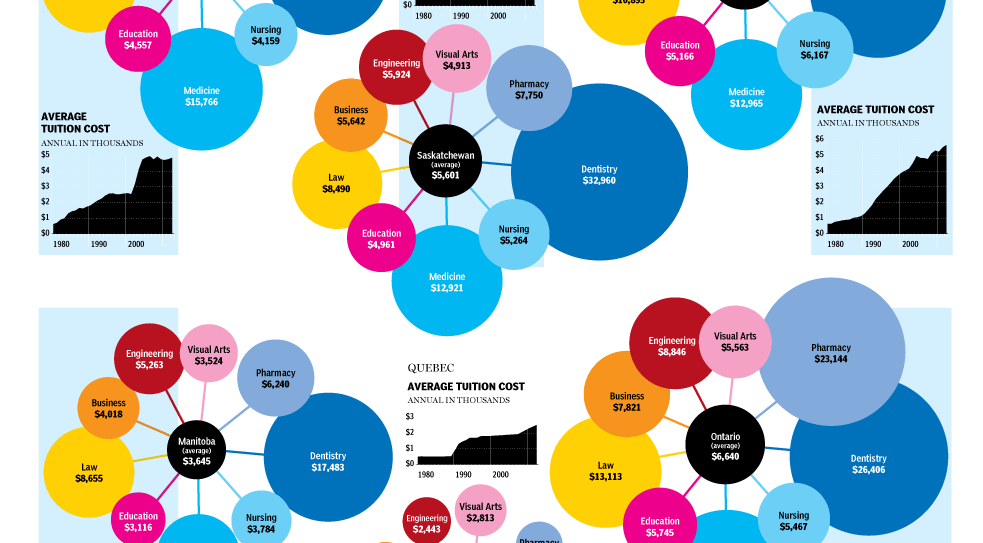
\includegraphics[keepaspectratio=TRUE,width=.9\linewidth]{junkcharts.png}
\end{frame}
\begin{frame}
    \frametitle{Motivation}
    \begin{itemize}
    \item Why are some plots easier to read?
    \hspace{-24pt}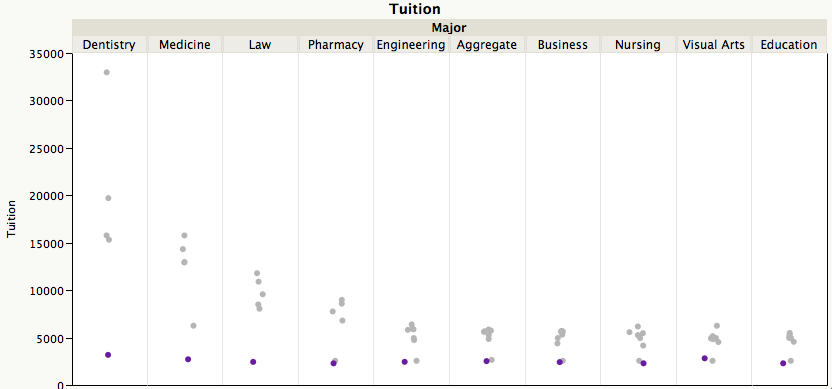
\includegraphics[keepaspectratio=TRUE,width=.9\linewidth]{dotplot.png}
    \item \url{http://junkcharts.typepad.com/junk_charts/2012/05/spring-flowers-and-striking-hours.html}
    \end{itemize}
\end{frame}

\begin{frame}
\frametitle{Good Graphics}
Graphics consist of 
\begin{itemize}
\item Structure (boxplot, scatterplot, etc.)
\item Aesthetics: features such as color, shape, and size that map other characteristics to structural features
\end{itemize}\bigskip
Both the structure and aesthetics should help viewers interpret the information.
\end{frame}

\begin{frame}
\frametitle{Outline}
\begin{itemize}
\item Cognitive aspects of perception and aesthetic choices\bigskip
\item Visual ordering mechanisms and color choices\bigskip
\item Faceting graphs to show additional variables\bigskip
\end{itemize}
\end{frame}


\begin{frame}
\frametitle{Pre-Attentive Features}
\begin{itemize}
\item Things that ``jump out" in less than 250 ms\medskip
\item Color, form, movement, spatial localization
\end{itemize}
\hfil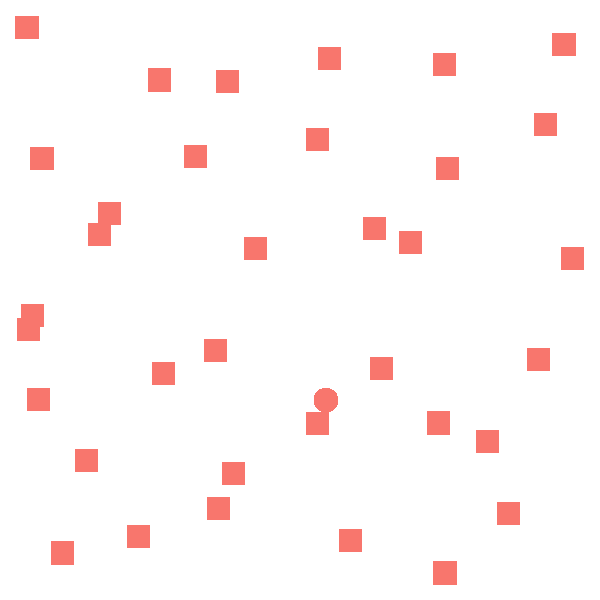
\includegraphics[width=.4\linewidth]{figure/preattentive11}\hspace{20pt}
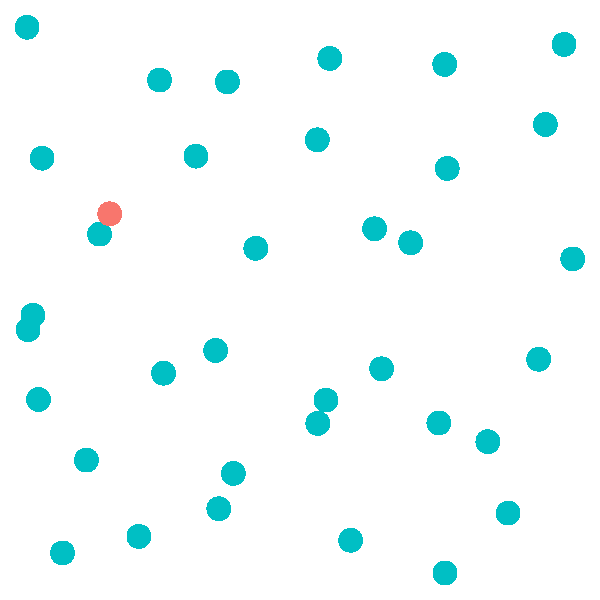
\includegraphics[width=.4\linewidth]{figure/preattentive12}
\end{frame}

% \begin{frame}
% \frametitle{Form}
% \begin{itemize}
% \item Size
% \item Angle
% \item Width
% \item Curvature
% \item Shape
% \item Length
% \item Grouping
% \item Added Marks
% \end{itemize}
% \end{frame}



\begin{frame}
\frametitle{Hierarchy of Features}
\begin{itemize}
\item Color is stronger than shape\medskip
\item Combinations of pre-attentive features are usually not pre-attentive due to \emph{interference}
\end{itemize}
\hfil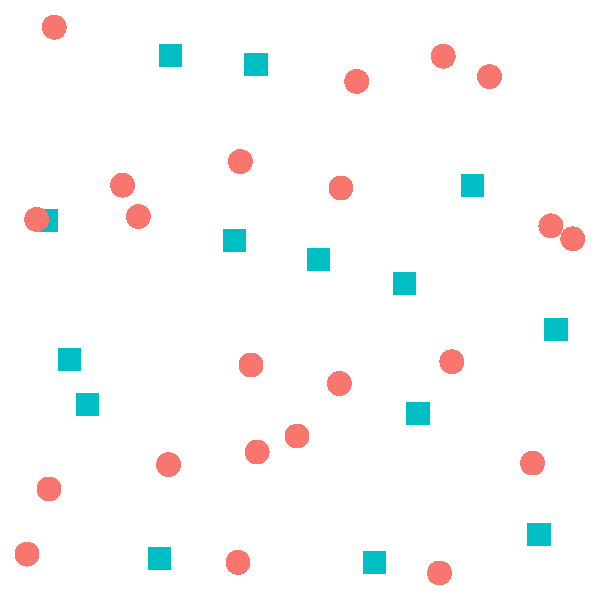
\includegraphics[width=.4\linewidth]{figure/preattentive21}\hspace{20pt}
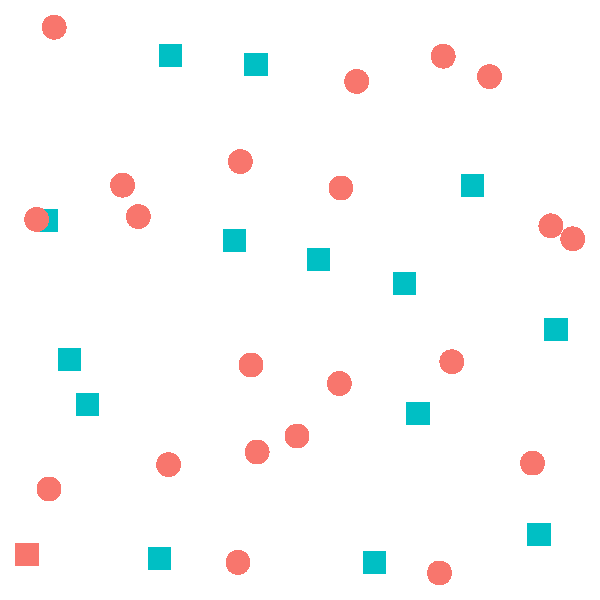
\includegraphics[width=.4\linewidth]{figure/preattentive22}
\end{frame}

\begin{frame}
\frametitle{Color}
\begin{itemize}
\item Hue: shade of color (red, orange, yellow...)
\item Intensity: amount of color
\item Both color and hue are pre-attentive. Bigger contrast corresponds to faster detection.
\end{itemize}
\begin{center}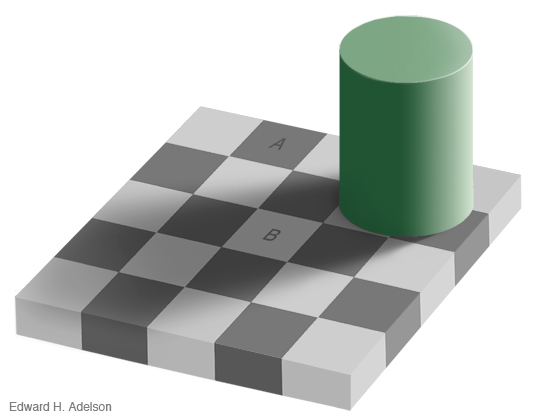
\includegraphics[keepaspectratio=TRUE,width=.3\textwidth]{shadowillusion}\end{center}
Color is context-sensitive: the exact same hue and intensity in one situation may appear to be a different color in a different context. A and B are the same intensity and hue, but appear to be different.
\end{frame}

\begin{frame}
\frametitle{Aesthetics in \texttt{ggplot2}}
\hfil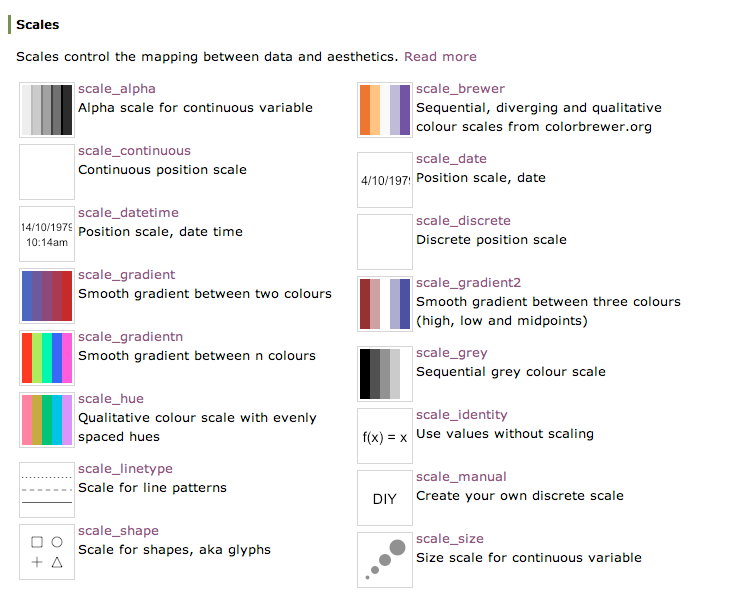
\includegraphics[width=.8\linewidth]{ggplot2aesthetics}\\
Main parameters: alpha, shape, color, size
\end{frame}

\begin{frame}[fragile]
\frametitle{Your Turn}
\vspace{-12pt}Find ways to improve the following graphic:
\begin{knitrout}\footnotesize
\definecolor{shadecolor}{rgb}{1, 1, 1}\color{fgcolor}\begin{kframe}
\begin{alltt}
\hlstd{frame} \hlkwb{<-} \hlkwd{data.frame}\hlstd{(}\hlkwc{x}\hlstd{=}\hlkwd{runif}\hlstd{(}\hlnum{25}\hlstd{),} \hlkwc{y}\hlstd{=}\hlkwd{runif}\hlstd{(}\hlnum{25}\hlstd{),}
        \hlkwc{g1}\hlstd{=}\hlkwd{rep}\hlstd{(}\hlkwd{c}\hlstd{(}\hlstr{"A"}\hlstd{,}\hlstr{"B"}\hlstd{),} \hlkwd{c}\hlstd{(}\hlnum{12}\hlstd{,}\hlnum{13}\hlstd{)),}
        \hlkwc{g2}\hlstd{=}\hlkwd{rep}\hlstd{(}\hlkwd{c}\hlstd{(}\hlstr{"1"}\hlstd{,} \hlstr{"2"}\hlstd{),} \hlkwd{c}\hlstd{(}\hlnum{13}\hlstd{,}\hlnum{12}\hlstd{)))}
\hlkwd{qplot}\hlstd{(x,y,} \hlkwc{shape}\hlstd{=g1,} \hlkwc{colour}\hlstd{=g2,} \hlkwc{data}\hlstd{=frame,} \hlkwc{size}\hlstd{=}\hlkwd{I}\hlstd{(}\hlnum{4}\hlstd{))}
\end{alltt}
\end{kframe}
\end{knitrout}
\vspace{-8pt}\begin{minipage}{.5\linewidth}
\begin{itemize}
\item Make sure the ``oddball" stands out while keeping the information on the groups
\item Hint: \texttt{interaction} combines factor variables
\end{itemize}
\end{minipage}
\begin{minipage}{.485\linewidth}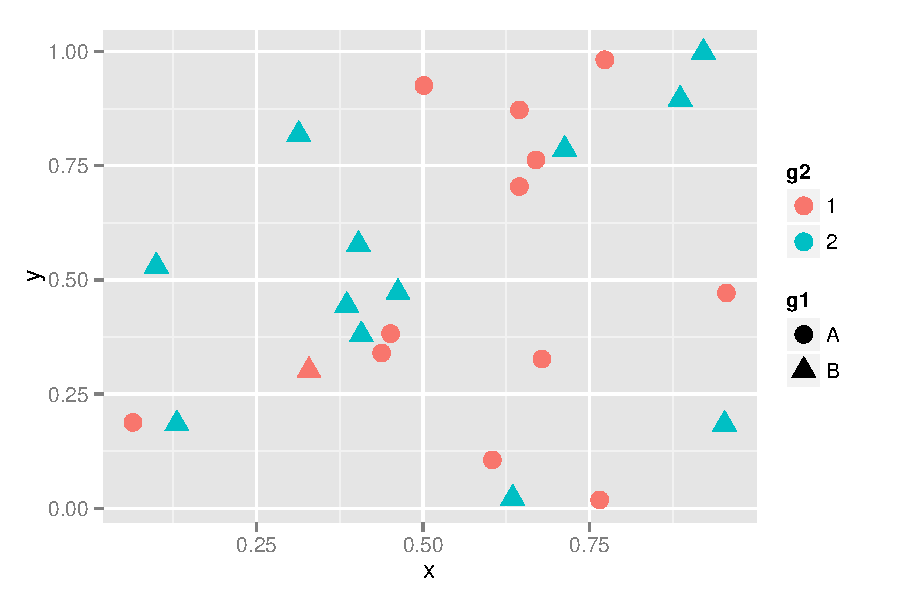
\includegraphics[width=.95\linewidth,keepaspectratio=TRUE]{figure/yourturn1}\end{minipage}
\end{frame}

\begin{frame}
\frametitle{Ordering Variables}
Which is bigger?
\begin{itemize}
\item Position: higher is bigger (y), items to the right are bigger (x)
\item Size, Area
\item Color: not always ordered. More contrast = bigger.
\item Shape: Unordered. 
\end{itemize}
\begin{center}
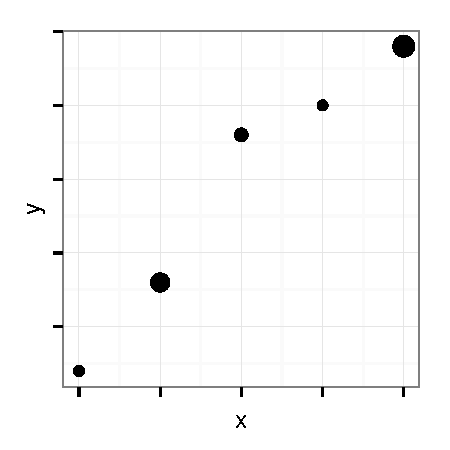
\includegraphics[width=.3\linewidth]{figure/ordering1}
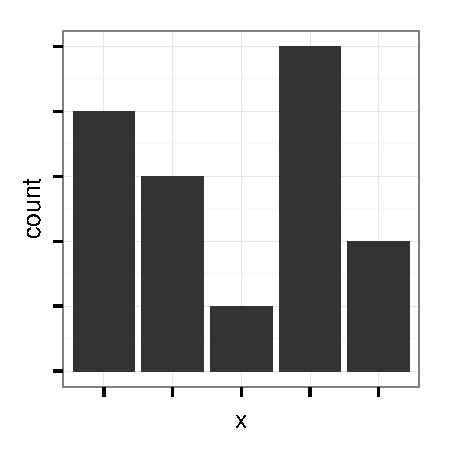
\includegraphics[width=.3\linewidth]{figure/ordering2}
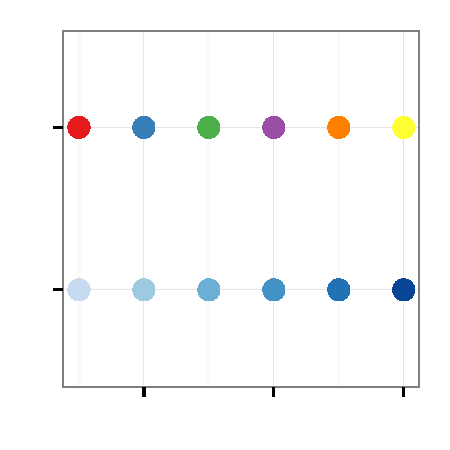
\includegraphics[width=.3\linewidth]{figure/ordering3}
\end{center}
\end{frame}



\begin{frame}
\frametitle{Using Color}
\begin{itemize}
\item Qualitative schemes: no more than 7 colors\\
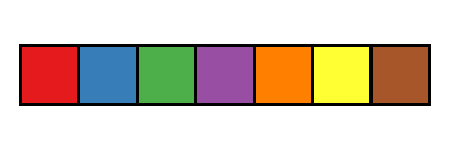
\includegraphics[width=.3\linewidth]{figure/gradients1}
\item Quantitative schemes: 
\begin{itemize}\item use color gradient with only one hue for positive values
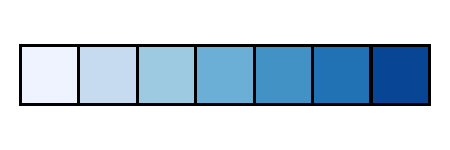
\includegraphics[width=.3\linewidth]{figure/gradients2}
\item use color gradient with two hues for positive and negative values. Gradient should go through a light, neutral color (white)\\
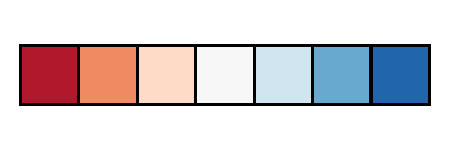
\includegraphics[width=.3\linewidth]{figure/gradients3}
\end{itemize}
\item Small objects or thin lines need more contrast than larger areas
\end{itemize}
\end{frame}

\begin{frame}[fragile]
\frametitle{RColorBrewer}
R package based on Cynthia Brewer's color schemes (\url{ColorBrewer2.org})\\
\begin{minipage}{.45\linewidth}
\begin{knitrout}\scriptsize
\definecolor{shadecolor}{rgb}{1, 1, 1}\color{fgcolor}\begin{kframe}
\begin{alltt}
\hlkwd{install.packages}\hlstd{(}\hlstr{"RColorBrewer"}\hlstd{)}
\hlkwd{library}\hlstd{(RColorBrewer)}
\hlkwd{help}\hlstd{(}\hlkwc{package}\hlstd{=RColorBrewer)}
\hlkwd{display.brewer.all}\hlstd{()}
\end{alltt}
\end{kframe}
\end{knitrout}
\end{minipage}
\begin{minipage}{.45\linewidth}
\begin{knitrout}\footnotesize
\definecolor{shadecolor}{rgb}{1, 1, 1}\color{fgcolor}

{\centering 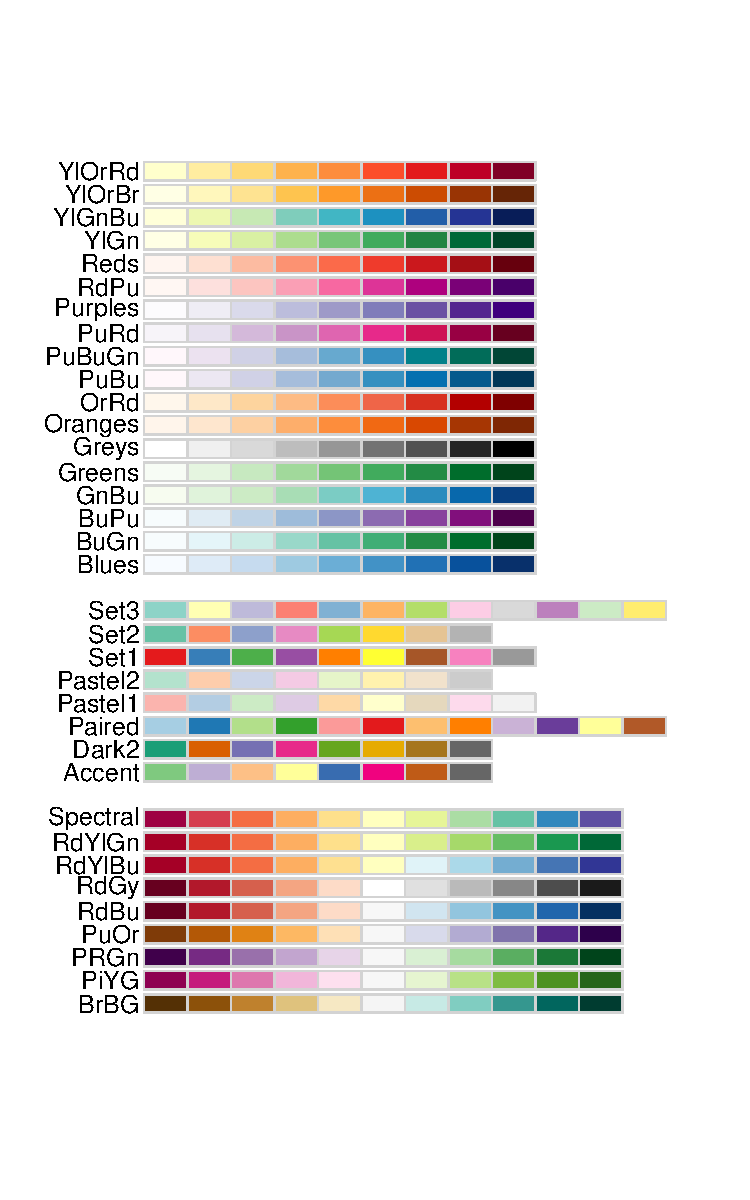
\includegraphics[width=.9\linewidth]{figure/brewerloadpic} 

}



\end{knitrout}
\end{minipage}
\end{frame}

\begin{frame}[fragile]
\frametitle{Color in ggplot2}
\begin{itemize}
\item factor variable: \\
\verb!scale_colour_discrete!\\
\verb!scale_colour_brewer(palette=...)!
\item continuous variable: \\
\verb!scale_colour_gradient! (define low, high values)\\
\verb!scale_colour_gradient2! (define low, mid, and high values)
\item equivalents for fill: \verb!scale_fill_...!
\end{itemize}
\end{frame}

\begin{frame}[fragile]
\frametitle{Your Turn}
\vspace{-12pt}
\small
\begin{itemize}
\item In the diamonds data, clarity and cut are ordinal, while price and carat are continuous
\item Find a graphic that gives an overview of these four variables while respecting their types
\item Hint: Start with \vspace{-4pt}
\begin{knitrout}\footnotesize
\definecolor{shadecolor}{rgb}{1, 1, 1}\color{fgcolor}\begin{kframe}
\begin{alltt}
\hlkwd{data}\hlstd{(diamonds)}
\hlkwd{qplot}\hlstd{(carat, price,} \hlkwc{shape}\hlstd{=cut,} \hlkwc{colour}\hlstd{=clarity,}
      \hlkwc{data}\hlstd{=diamonds)}
\end{alltt}
\end{kframe}

{\centering 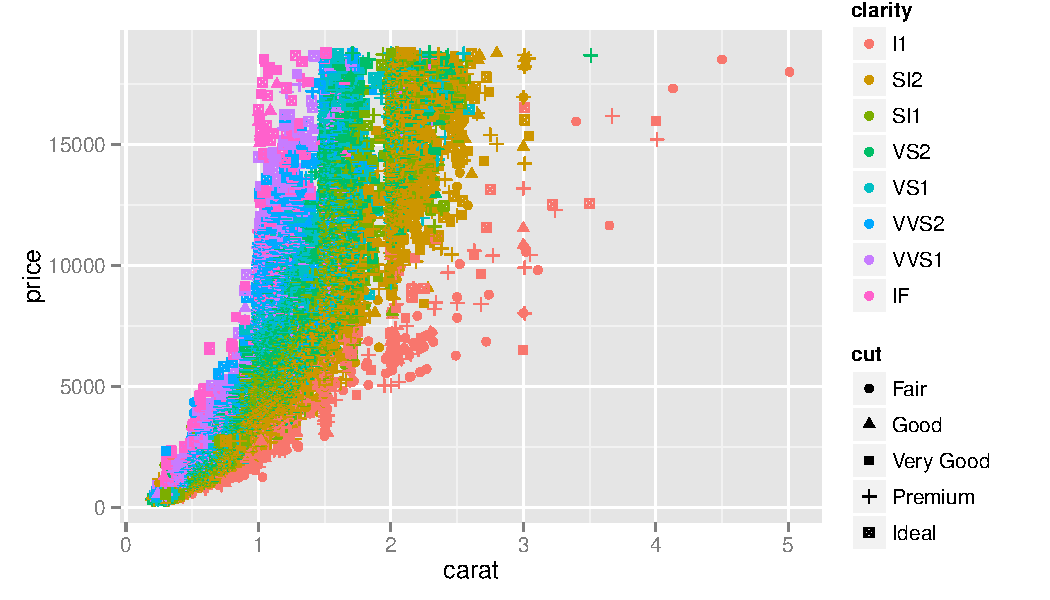
\includegraphics[width=.55\linewidth]{figure/yourturn2} 

}



\end{knitrout}
\vspace{-6pt}
% \item It may be helpful to try \verb#qplot() + facet_wrap(~cut)#
\end{itemize}
\end{frame}

\begin{frame}[fragile]
\frametitle{Facetting}
\begin{itemize}
\item A way to extract subsets of data and place them side-by-side in graphics
\item Syntax: \verb#facets = row ~ col# Use \texttt{.} if there is no variable for either row or column (i.e. \verb#facets = . ~ col#)
\begin{knitrout}\scriptsize
\definecolor{shadecolor}{rgb}{1, 1, 1}\color{fgcolor}\begin{kframe}
\begin{alltt}
\hlkwd{qplot}\hlstd{(price, carat,} \hlkwc{data}\hlstd{=diamonds,} \hlkwc{color}\hlstd{=color,}
      \hlkwc{facets} \hlstd{= .} \hlopt{~} \hlstd{clarity)}
\end{alltt}
\end{kframe}
\end{knitrout}
\begin{knitrout}\footnotesize
\definecolor{shadecolor}{rgb}{1, 1, 1}\color{fgcolor}

{\centering 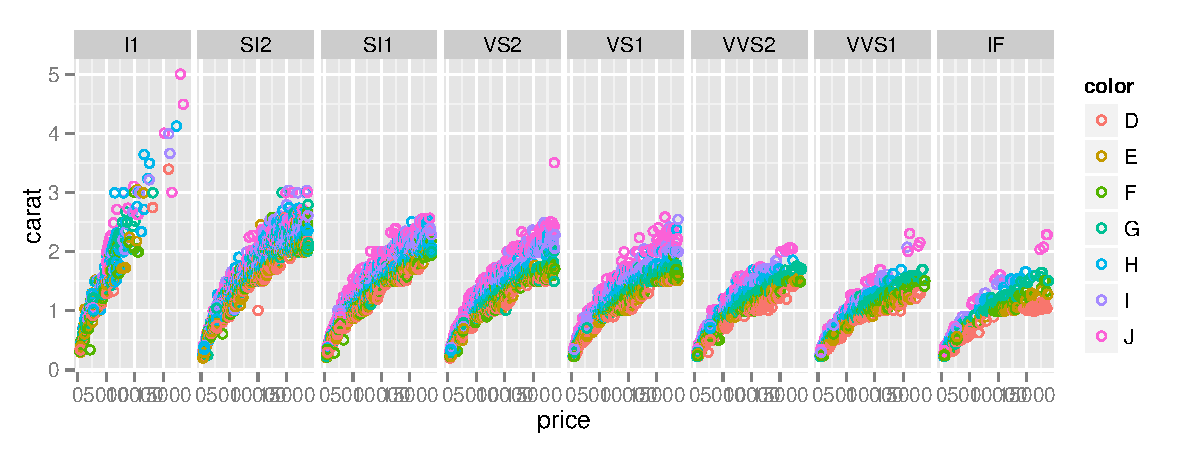
\includegraphics[width=\linewidth]{figure/diamondsdemo2} 

}



\end{knitrout}
\end{itemize}
\end{frame}


\begin{frame}
\frametitle{Your Turn}
\begin{itemize}
\item The \texttt{movies} dataset contains information from IMDB.com including ratings, genre, length in minutes, and year of release. \medskip
\item Explore the differences in length, rating, etc. in movie genres over time \medskip
\item Hint: use facetting!
\end{itemize}
\end{frame}

\end{document}
